\documentclass[hyperref = {unicode},aspectratio = 169]{beamer}
\mode<presentation>
\usepackage[utf8]{inputenc}				% native UTF-8 characters in file
\usepackage{amssymb}							% maths symbols
\usepackage{mathtools}						% loads and improves amsmath
\usepackage{amsthm}								% theorems
\usepackage{thmtools,thm-restate}	% theorem improvements
\usepackage{graphicx}							% loading pictures
\usepackage{silence}							% suppressing warnings
\usepackage{tikz-cd}							% commutative diagrams
\usetikzlibrary{babel}						% allows maths inside tikzcd env
\usepackage{parskip}							% space between paragraphs
\usepackage{mleftright}						% slimmer auto-delimiter spacing

\hypersetup{
	% colorlinks = true,
	linkcolor = blue,
	citecolor = green,
	urlcolor = black
}

\declaretheorem{proposition}

\setlength{\parskip}{6pt plus 2pt minus 2pt}

\graphicspath{{./images/}}

% use special characters instead of numbers for footnotemarks:
\renewcommand{\thefootnote}{\fnsymbol{footnote}}

\hfuzz = 5pt
\newdimen\hfuzz	% for ignoring small overfull hbox's

\definecolor{uibred1}{RGB}{180, 50, 100}
\definecolor{uibred}{RGB}{100, 0, 0}
\definecolor{uibblue}{RGB}{0, 84, 115}
\definecolor{uibgreen}{RGB}{119, 175, 0}
\definecolor{uibgreen1}{RGB}{50, 105, 0}
\definecolor{uiborange}{RGB}{217, 89, 0}

\setbeamertemplate{blocks}[rounded][shadow = false]
\addtobeamertemplate{block begin}{\pgfsetfillopacity{0.8}}{\pgfsetfillopacity{1}}
\setbeamercolor{structure}{fg = uibred}
\setbeamercolor*{block title example}{fg = white,bg = uibred}
\setbeamercolor*{block body example}{fg = black,bg = uibred!10}

%% custom commands
% primed operators
% TeXbook 18.44
\def\p[#1]_#2{
	\setbox0 = \hbox{$\scriptstyle{#2}$}
	\setbox2 = \hbox{$\displaystyle{#1}$}
	\setbox4 = \hbox{${}'\mathsurround = 0pt$}
	\dimen0 = .5\wd0 \advance\dimen0 by-.5\wd2
	\ifdim\dimen0>0pt
	\ifdim\dimen0>\wd4 \kern\wd4 \else\kern\dimen0\fi\fi
	\mathop{{#1}'}_{\kern-\wd4 #2}
}
\def\sump_#1{\p[\sum]_{#1}}
\def\prodp_#1{\p[\prod]_{#1}}
\def\minp_#1{\p[\min]_{#1}}
\def\maxp_#1{\p[\max]_{#1}}
% sets
\newcommand*{\NN}{\mathbb{N}}
\newcommand*{\NNO}{\mathbb{N}_0}
\newcommand*{\ZZ}{\mathbb{Z}}
\newcommand*{\QQ}{\mathbb{Q}}
\newcommand*{\RR}{\mathbb{R}}
\newcommand*{\CC}{\mathbb{C}}
\newcommand*{\CCi}{\mathbb{C}_\infty}
\newcommand*{\HH}{\mathcal{H}}
\newcommand*{\FF}{\mathbb{F}}
\newcommand*{\PP}{\mathbb{P}}
\newcommand*{\LL}{\mathcal{L}}
\renewcommand{\AA}{\mathbb{A}}
\newcommand*{\cJ}{\mathcal{J}}
\newcommand*{\finadele}{\AA_F^{fin}}
\newcommand*{\invertadele}{\bigl(\finadele\bigr)^{\!\times}}
\newcommand*{\fp}{\mathfrak{p}}
\newcommand*{\WeakMF}{\mathfrak{W}}
\newcommand*{\StrongMF}{\mathfrak{M}}
\newcommand*{\CuspMF}{\mathfrak{S}}
\newcommand*{\cw}{\mathcal{W}}
\newcommand*{\cm}{\mathcal{M}}
\newcommand*{\cs}{\mathcal{S}}
\newcommand*{\LLi}[2]{\protect\overleftarrow{\LL_{#1}^{#2}}}
\newcommand*{\LLNRi}{\LLi{N}{r}}
% arrows
% \newcommand*{\isoto}{\overset{\sim}{\to}}
\newcommand*{\isoto}{\xrightarrow{\mathmakebox[1.5ex]{\sim}}}
\newcommand*{\into}{\hookrightarrow}
\newcommand*{\onto}{\twoheadrightarrow}
\newcommand*{\ionto}{\lhook\joinrel\twoheadrightarrow}
\newcommand*{\xinto}[2][]{\xhookrightarrow[#1]{#2}}
\newcommand*{\xonto}[2][]{\xrightarrow[#1]{#2}\mathrel{\mkern-14mu}\rightarrow}
\newcommand*{\xionto}[2][]{\xhookrightarrow[#1]{#2}\mathrel{\mkern-22mu}\rightarrow\mathrel{\mkern6mu}}
\newcommand*{\mapsfrom}{\mathrel{\reflectbox{\ensuremath{\mapsto}}}}
% maths operators
\DeclareMathOperator{\End}{End}
\DeclareMathOperator{\B}{B}
\DeclareMathOperator{\D}{D}
\DeclareMathOperator{\Cl}{Cl}
\let\Im = \relax \DeclareMathOperator{\Im}{Im}
\DeclareMathOperator{\Sur}{Sur}
\DeclareMathOperator{\Inj}{Inj}
\DeclareMathOperator{\Free}{Free}
\DeclareMathOperator{\GLL}{GL}
\newcommand*{\GL}[2][]{\GLL_{#1}\parens{#2}}
\DeclareMathOperator{\SLL}{SL}
\newcommand*{\SL}[2][]{\SLL_{#1}\parens{#2}}
\DeclareMathOperator{\Div}{Div}
\DeclareMathOperator{\bd}{\partial}
% differentiation
\newcommand*{\dd}{\operatorname{d}}
\newcommand*{\id}[1]{\,\dd{#1}}
\newcommand*{\dbd}[2][]{\frac{\dd^{#1}}{\dd\!#2^{#1}}}
% enclosures
\mleftright	% fixes spacing around left-(middle-)right delimiters
% \delimiterfactor = 851
\delimitershortfall = 10pt
\newcommand*{\set}[1]{\left\{#1\right\}}
\newcommand*{\setst}[2]{\left\{#1\:\middle|\:#2\right\}}
\newcommand*{\order}[1]{\!O\!\left(#1\right)\!}
\newcommand*{\norm}[1]{\left\lVert 1\right\rVert}
\newcommand*{\abs}[1]{\left\lvert#1\right\rvert}
\newcommand*{\floor}[1]{\left\lfloor#1\right\rfloor}
\newcommand*{\ceil}[1]{\left\lceil#1\right\rceil}
\newcommand*{\fracpart}[1]{\left\{#1\right\}}
\newcommand*{\parens}[1]{\left(#1\right)}
\newcommand*{\pparens}[1]{\parens{\!\parens{#1}\!}}
\newcommand*{\brackets}[1]{\left[#1\right]}
\newcommand*{\braces}[1]{\left\{#1\right\}}
\newcommand*{\size}{\#}
\newcommand*{\sizep}[1]{\size\parens{#1}}
\newcommand*{\sizeset}[1]{\size\set{#1}}
\newcommand*{\sizesetst}[2]{\size\setst{#1}{#2}}
\newcommand*{\lquotient}[2]{\left. #1 \middle\backslash #2 \right.}
\newcommand*{\rquotient}[2]{\left. #1 \middle/ #2 \right.}
\newcommand*{\lrquotient}[3]{\left. #1 \middle\backslash #2 \middle/ #3 \right.}
\newcommand*{\cin}[2]{\bigl[{#1}^{#2}\bigr]}
\newcommand*{\bigO}[1]{\mathcal{O}\parens{#1}}
\newcommand*{\littleo}[1]{o\parens{#1}}
\newcommand*{\pcoord}[1]{%
  \begingroup\lccode`~ = `: \lowercase{\endgroup
  \edef~}{\mathbin{\mathchar\the\mathcode`:}\nobreak}%
  \left(% opening symbol
  \begingroup
  \mathcode`: = \string"8000
  #1%
  \endgroup
  \right)% closing symbol
}
% maths text spacing
\newcommand*{\lrsptext}[1]{\quad\text{#1}\quad}
\newcommand*{\lsptext}[1]{\quad\text{#1}\ }
\newcommand*{\rsptext}[1]{\ \text{#1}\quad}
\newcommand*{\sptext}[1]{\ \text{#1}\ }
% other
\newcommand*{\ie}{i.e.\ }
\newcommand*{\eqtag}{\stepcounter{equation} \tag{\theequation}}
\newcommand*{\defeq}{\coloneqq}
\newcommand*{\eqdef}{\eqqcolon}



\mode<presentation>{
  \usetheme{ift}
  %\setbeamercovered{transparent}	% commented because it messes with uncovering lines in align environments
  \setbeamertemplate{items}[square]
}

\usefonttheme[onlymath]{serif}
\setbeamerfont{frametitle}{size = \Large}
\setbeamertemplate{navigation symbols}{}
% \AtBeginSection[]{
% 	\begin{frame} \vfill \centering
% 	\begin{beamercolorbox}[sep = 8pt,center]{title}
% 		\usebeamerfont{title}Chapter~\thesection \\\vspace{12pt} \insertsectionhead\par
% 	\end{beamercolorbox}
% 	\vfill \end{frame}
% }

\title[Drinfeld modular forms]
  {\LARGE Drinfeld modular forms}
\subtitle{\large IAS Short Talk}
\author[Liam Baker]{Liam Baker}
\date[2023/10/05]{5 October 2023}
\institute[Stellenbosch University]{Department of Mathematical Sciences \\ Stellenbosch University}


\begin{document}

\setbeamertemplate{background}{
  
\includegraphics[width = \paperwidth, height = \paperheight]{frontpage_bg_169}
}
\setbeamertemplate{footline}[default]
\begin{frame}
  \titlepage
\end{frame}


\setbeamertemplate{background}{
  
\includegraphics[width = \paperwidth, height = \paperheight]{slide_bg_169}
}
\setbeamertemplate{footline}[ifttheme]

\section{Classical Modular Forms}


\subsection{These are pretty cool!}

\begin{frame} \frametitle{Classical modular forms -- Definition 1}
  Modular forms are analytic functions on the complex upper half plane which have important number theoretical properties. \pause
  \begin{definition}
    A (classical) modular form $f$ of weight $k \in \NNO$ for the group $\SL[2]{\ZZ}$ is a function on the complex upper half plane $\HH = \setst{z \in \CC}{\Im{z} > 0}$ satisfying the following properties: \pause
    \begin{itemize}
      \item $f$ is complex analytic on $\HH$\pause,
      \item $f\parens{\frac{az+b}{cz+d}} = (cz+d)^{k} f(z)$ for all $a,b,c,d \in \ZZ$ such that $ad-bc = 1$\pause, and
      \item $\abs{f(z)}$ is bounded as $\Im{z} \to +\infty$.\pause \hfill \emph{(holomorphic at infinity)}
    \end{itemize}
  \end{definition}

  The second condition can be written as $f(\gamma z) = j(\gamma,z)^{-k} f(z)$ for all $\gamma = \parens{\begin{smallmatrix} a & b \\ c & d \end{smallmatrix}} \in \SL[2]{\ZZ}$, with \emph{factor of automorphy} $j(\gamma,z) = cz+d$.
\end{frame}


\begin{frame} \frametitle{Classical modular forms -- Definition 1}
  Here the group $\SL[2]{\ZZ}$ acts on $\HH$ from the left by the fractional linear transformation $z \xmapsto{\gamma} \frac{az+b}{cz+d}$, which is closely related to matrix multiplication on the left:
  \[ \begin{pmatrix} a & b \\ c & d \end{pmatrix} \begin{pmatrix} z \\ 1 \end{pmatrix} = \begin{pmatrix} az+b \\ cz+d \end{pmatrix} = \frac{1}{cz+d} \begin{pmatrix} \frac{az+b}{cz+d} \\ 1 \end{pmatrix}. \]
  \pause
  The left action of $\SL[2]{\ZZ}$ on $\HH$ translates into a right action on the functions $f : \HH \to \CC$:
  \[ f|_\gamma : \HH \to \CC, \quad z \mapsto j(\gamma,z)^{-k} f(\gamma z) = (cz+d)^{-k} f\parens{\frac{az+b}{cz+d}}. \]
  \pause
  The transformation condition in the previous definition can then be restated more simply: \pause
  \[ f|_\gamma(z) = f(z) \lsptext{for all} \gamma \in \SL[2]{\ZZ}. \]
\end{frame}


\begin{frame} \frametitle{Classical modular forms -- Definition 1}
  The first definition above is that of a modular form for the \emph{full} group $\SL[2]{\ZZ}$.
  More generally, for any $N \in \NN$ we can define a modular form for any \emph{congruence subgroup} $\Gamma \subseteq \SL[2]{\ZZ}$:
  \[ \Gamma \supseteq \Gamma(N) = \setst{\parens{\begin{smallmatrix} a & b \\ c & d \end{smallmatrix}} \in \SL[2]{\ZZ}}{\parens{\begin{smallmatrix} a & b \\ c & d \end{smallmatrix}} \equiv \parens{\begin{smallmatrix} 1 & 0 \\ 0 & 1 \end{smallmatrix}} \pmod{N}}: \pause \]
  \begin{definition}
    A modular form $f$ of weight $k$ for the congruence subgroup $\Gamma$ is a function $f : \HH \to \CC$ such that: \pause
    \begin{itemize}
      \item $f$ is complex analytic on $\HH$\pause,
      \item $f|_\gamma(z) = f(z)$ for all $\gamma \in \Gamma$\pause, and
      \item $\abs{f|_\gamma(z)}$ is bounded as $\Im{z} \to +\infty$ for all $\gamma \in \SL[2]{\ZZ}$. \pause \hfill \emph{(holomorphic at the cusps)}
    \end{itemize}
  \end{definition} \pause

  % Note that if $\Gamma = \Gamma(1) = \SL[2]{\ZZ}$, we get a modular form for the full group $\SL[2]{\ZZ}$.
\end{frame}


\subsection{A function on lattices?}

\begin{frame} \frametitle{Classical modular forms -- Definition 2}
  An alternative way to define a modular form is as a function on the space $\LL$ of lattices of rank $2$\pause; here a lattice (of rank $2$) is a free rank-$2$ additive subgroup $\Lambda = a\ZZ +b\ZZ \subset \CC$:\pause

  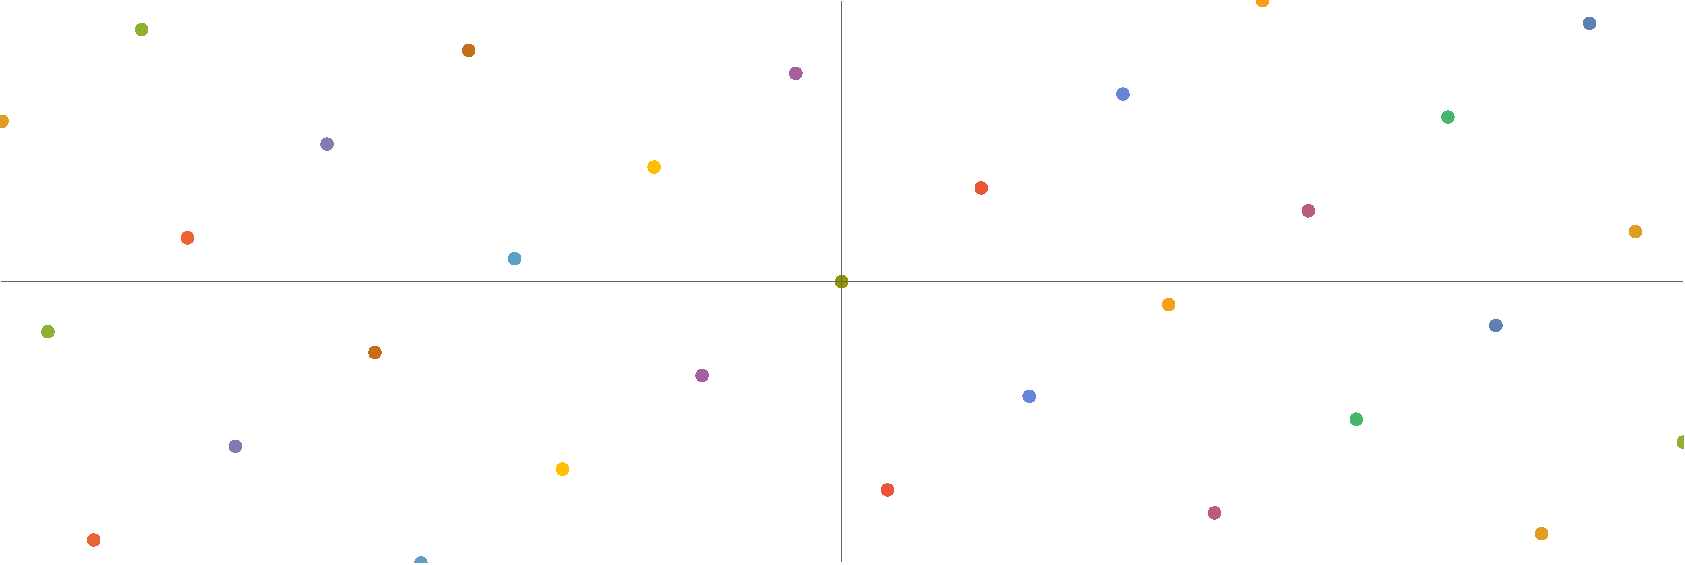
\includegraphics[width = \textwidth]{lattice.pdf}
\end{frame}


\begin{frame} \frametitle{Classical modular forms -- Definition 2}
  \begin{definition}
    A modular form $f$ of weight $k$ for $\SL[2]{\ZZ}$ is a function $f : \LL \to \CC$ such that:
    \begin{itemize}
      \item $f$ is analytic\pause, \hfill (?) \pause
      \item $f$ is homogeneous of degree $-k$: \pause $f(r\Lambda) = r^{-k} f(\Lambda)$ for all $r \in \CC^\times$ and $\Lambda \in \LL$\pause, and
      \item $\abs{f(\Lambda)}$ is bounded as long as the smallest element of $\Lambda$ is bounded away from $0$.\pause
    \end{itemize}
  \end{definition}

  If $f$ is a modular form in this lattice sense, then $\bar{f}(z) = f(z\ZZ+\ZZ)$ is a modular form in the complex-variable sense.
  In fact, the converse is also true, so that these two definitions are equivalent. \pause

  To define a modular form for the congruence subgroup $\Gamma(N)$ as a function of lattices we actually define it as a homogeneous function $f(\Lambda,\alpha)$ of a lattice $\Lambda$ together with a \emph{level structure} $\alpha : N^{-1}\Lambda/\Lambda \ionto (N^{-1}/\ZZ)^2$.
\end{frame}

\section{Drinfeld modular forms}


\subsection{Set the stage}

\begin{frame} \frametitle{The Drinfeld setting}
  We now move from the classical setting to that of function field arithmetic.
  % Most of the data are analogous with more familiar objects:

  \uncover<8->{\makebox[14mm][l]{} \textbar} \textbf{Function field object} \hfill \textbf{Classical analogue} \pause \\
  \uncover<8->{\makebox[14mm][l]{$\FF_q(T)$} \textbar} $F$, a fixed global function field \hfill $\QQ$, the rational numbers \pause \\
  \uncover<8->{\makebox[14mm][l]{} \textbar} $\abs{\cdot}$, an absolute value on $F$ with place $\infty$ \hfill the usual absolute value $\abs{\cdot}$ on $\CC$ \pause \\
  \uncover<8->{\makebox[14mm][l]{$\FF_q[T]$} \textbar} $A$, the ring of elements of $F$ regular away from $\infty$ \hfill $\ZZ$, the integers \pause \\
  \uncover<8->{\makebox[14mm][l]{$\FF_q((\frac{1}{T}))$} \textbar} $\FF_\infty$, the completion of $F$ with respect to $\abs{\cdot}$ \hfill $\RR$, the real numbers \pause \\
  \uncover<8->{\makebox[14mm][l]{} \textbar} $\CC_\infty$, the completion of an algebraic closure of $\FF_\infty$ \hfill $\CC$, the complex numbers \pause

  Here, analogously with the classical setting, $A$ is a Dedekind ring.
  We also consider the positive integer $q$, which is the cardinality of the field of constants of $F$, with associated finite field $\FF_q$.
\end{frame}


\subsection{The only constant is change}

\begin{frame} \frametitle{Differences to the classical setting}
  In contrast with the classical setting, there are some key differences: \pause
  \begin{itemize}
    \item The main rings are of finite characteristic, and the absolute value $\abs{\cdot}$ is \emph{non-archimedean}; hence analytic issues such as convergence of series are in some ways easier, whereas defining an analytic function is more complex than in the classical case. \pause
    % \item As previously mentioned, lattices can have arbitrarily high integer rank. \pause
    \item We do not generally have factorisation of elements of $A$ into products of prime elements and ideals are not always principal. However, since $A$ is a Dedekind ring we do have unique factorisation of \emph{ideals} into products of prime ideals. \pause So we henceforth let $N$ be an arbitrary proper ideal of $A$. \pause
    \item Here $\CC_\infty$ has \emph{infinite} dimension as a vector space over $\FF_\infty$, whereas $\CC$ has dimension $2$ as a vector space over $\RR$. \pause
    As a result, whereas lattices in the classical case can have rank at most $2$, here lattices can have arbitrarily high rank. This what makes the theory of `modular forms of higher rank' possible.
  \end{itemize}
\end{frame}


\subsection{What am I even doing?}

\begin{frame} \frametitle{My work -- higher rank modular forms}
  Whereas most of the theory of Drinfeld modular forms has focused on modular forms of rank $2$, due to the simplicity of dealing with a function of one variable and on analogy with the classical case, recent work by Gekeler (for $F = \FF_q(T)$) and Basson, Breuer, and Pink (for general $F$) have established theories of Drinfeld modular forms of higher rank. \pause
  
  Their approach has been viewing them as functions of $r-1$ variables, whereas my PhD thesis establishes a theory viewing them as functions on the space of lattices of higher rank. \pause
  My current work in this area is on further filling out the theory from this point of view.

  % Additionally, in the rank 2 case there is the question of generators for the (graded) algebra of modular forms for the principal congruence subgroup $\Gamma(N)$, where I have some partial computational results.
\end{frame}


\begin{frame} \frametitle{Lattices}
  \begin{definition}
    A lattice $\Lambda$ of rank $r$ is a projective $A$-submodule of $\CC_\infty$ of rank $r$ \pause (\ie a subset of $\CC_\infty$ of the form $I_1\psi_1 +\dotsb +I_r\psi_r$ for ideals $I_i \subseteq A$ and $\psi_i \in \CC_\infty$ which are $\FF_\infty$-linearly independent). \pause

    A level $N$ structure for a lattice $\Lambda$ of rank $r$ is an $A$-module bijection $\parens{N^{-1}/A}^r \ionto N^{-1}\Lambda/\Lambda$.
  \end{definition} \pause

  % Every lattice has $\size{\GL[r]{A/N}}$ different level $N$ structures, since $A$ is a Dedekind ring.

  We denote the space $\set{(\Lambda,\alpha)}$ of lattices $\Lambda$ of rank $r$ with level $N$ structure $\alpha$ by $\LL_N^r$, and the space of lattices $\Lambda$ of rank $r$ without level structure by $\LL^r$. \pause
  % The left action of $\gamma \in \GL[2]{A/N}$ on $\LL_N^r$ is given by
  % \[ \gamma(\Lambda,\alpha) \defeq (\Lambda, \alpha \circ \gamma^{-1}). \]

  We prove that these spaces are rigid analytic spaces by identifying them with a double quotient:
  \[ \LL_N^r \simeq \left. \GL[r]{F} \middle\backslash \parens{\Psi^r \times \GL[r]{\AA_F^{fin}}/K(N)} \right. \]
  and so we can speak of holomorphic functions on these spaces.
\end{frame}


\begin{frame} \frametitle{Higher rank modular forms} \pause
  We define metrics $\dd_\LL$ and $\dd_{\LL_N^r}$ on the rigid analytic spaces $\LL^r$ and $\LL_N^r$, leading to their completions $\LL^{\leq r}$ and $\LLNRi$, where the boundaries consist of spaces of lattices of lower rank. \pause
  \begin{definition} \label{def:strongMForm}
    A \emph{modular form} of \emph{weight} $k$ and \emph{rank} $r$ for $K(N)$ is a function $f : \LLNRi \to \CCi$ which is: \pause
    \begin{itemize}
      \item holomorphic on the interior $\LL_N^r$ of $\LLNRi$\pause,
      \item homogeneous of degree $-k$\pause, and
      \item continuous on $\LLNRi$. \pause
    \end{itemize}
  \end{definition}

  % The left action of $\gamma \in \GL[2]{A/N}$ on $\LLNRi$ translates to a right action on the space of modular forms, by $f|_\gamma(\Lambda,\alpha) = f(\Lambda, \alpha \circ \gamma^{-1})$.

  My PhD thesis established the general theory of modular forms of higher rank as functions of lattices, and I am currently extending this theory in the following areas: \pause
  \begin{itemize}
    \item Proving that modular forms have Fourier-type series expansions at cusps\pause, and
    \item Defining Hecke operators and proving their recursive properties.
  \end{itemize}
\end{frame}


\begin{frame} \frametitle{My work -- Eisenstein series in rank $2$} \pause
  Typical examples of modular forms of rank $2$ for $\Gamma(N)$ are the (partial) Eisenstein series:
  \[ E_{r_1,r_2}(z) = \sum_{m,n \in A} \frac{1}{(m+r_1)z+n+r_2} \lsptext{for} r_1,r_2 \in N^{-1}A/A; \]
  which are forms of weight $1$. \pause

  Cornelissen proved that in the case of $A = \FF_q[T]$ the graded algebra of Drinfeld modular forms of rank $2$ for $\Gamma(N)$ are generated by these Eisenstein series and possibly some cusp forms of weight $2$, but it is not known whether or not these cusp forms are necessary. \pause
  
  I have some partial computational results in this direction: for specific $N$ we can reduce it to linear algebra using the series expansions of these Eisenstein series at the cusps and the known dimension of the space of weight $2$ modular forms, but I hope to finish it off analytically.
\end{frame}

\include{d_3_lattices}

\include{d_4_modular_forms}





\end{document}